\documentclass[10pt,journal]{IEEEtran}
\usepackage{cite, graphicx, subfigure, amsmath} 
\usepackage{algorithm, algorithmic}
\usepackage{graphicx}
\interdisplaylinepenalty=2500

% *** Do not adjust lengths that control margins, column widths, etc. ***
% *** Do not use packages that alter fonts (such as pslatex).         ***
% There should be no need to do such things with IEEEtran.cls V1.6 and later.


\begin{document}
% paper title
\title{Parallelizing k-means}


% author names and IEEE memberships
% note positions of commas and nonbreaking spaces ( ~ ) LaTeX will not break
% a structure at a ~ so this keeps an author's name from being broken across
% two lines.
% use \thanks{} to gain access to the first footnote area
% a separate \thanks must be used for each paragraph as LaTeX2e's \thanks
% was not built to handle multiple paragraphs
\author{Chris Jordan,
Victor Janmey,
and Raymond W. Ko}% <-this % stops a space


% The paper headers
%\markboth{<+Journal of VIM-\LaTeX\ Class Files,~Vol.~1, No.~8,~August~2002+>}{
%<+Bhardwaj \MakeLowercase{\textit{et al.}+>}: <+Skeleton of IEEEtran.cls for Journals in VIM-Latex+>}
% The only time the second header will appear is for the odd numbered pages
% after the title page when using the twoside option.


% If you want to put a publisher's ID mark on the page
% (can leave text blank if you just want to see how the
% text height on the first page will be reduced by IEEE)
%\pubid{0000--0000/00\$00.00~\copyright~2002 IEEE}


% use only for invited papers
%\specialpapernotice{(Invited Paper)}


% make the title area
\maketitle

\begin{abstract}
Abstract goes where? Abstract goes here!
\end{abstract}

\begin{keywords}
k-means, parallel programming.
\end{keywords}

\section{Introduction}
\PARstart{T}{he} k-means algorithm groups particles into a fixed number of clusters.
It has an extraordinary amount of uses including in fields such as
machine learning, computer vision, and network analysis.

In the case of machine learning, it is useful in unsupervised learning methods, 
dividing data for more specific classifiers, and the selection of of examples for k-nearest neighbors.

For computer vision, one frequest task is to segment images using the difference in pixel intensity as a distance
metric. One can then use the k-means algorithm to do the above and estimate object boundaries, or use it as a cue for other algorithms
that perform object recognition.

Additinally, the use of k-means is not limited to just images, in network analysis it can be used to find communities.

However, in this paper, we will focus on the problem of image segmentation, in which which we will try to tune the code
to run as fast as possible.

\section{Analysis of Algorithm}
Before focusing on the acutal implementation, the k-means algorithm
was examined to see what sections could be effectively parallelized.

\subsection{\textit{k-means}}
The k-means algorithm basically consists of three steps:
choosing $k$ intial clusters, an assignment step, and an
update step. In the assignement step, particles get assigned
to clusters. In the update step, the new mean of a cluster
is recomputed by the making the average of all the values
of the particles in a cluster.

\begin{algorithm}
\caption{k-means++ algorithm}
\begin{algorithmic}[1]
\STATE{choose $k$ initial means as centers}
\FOR{each particle $p$}
    \FOR{each mean $k$}
        \STATE{calculate distance from $p$ to $k$}
        \IF {distance $<$ previous calculated distance}
            \STATE{mark down mean}
        \ENDIF
    \ENDFOR
    \STATE{put $k$ into last marked down cluster with mean}
\ENDFOR
\FOR{each cluster $c$}
    \STATE{sum $\leftarrow$ 0}
    \FOR{each partice $p$ in $c$}
        \STATE{sum $\leftarrow$ sum $+$ p}
    \ENDFOR
    \STATE{new mean of cluster $c$ $\leftarrow$ sum / $|c|$}
\ENDFOR
\STATE{repeat steps 2 to 17 until new means converge and no longer change}
\end{algorithmic}
\end{algorithm}

An initial and precursory glance at the algorithm indicates that there are parts that are
easy to parallelize.

The initial steps for choosing $k$ can be done in any fashion, and since they are not
dependent on each other, can simply be randomly chosen in parallel.

The second step, the assignment step, is the time dominating factor in the calculation since
it is $O(kn)$ due to the fact that for every particle, it must consider every $k$-clusters.
Nevertheless, since the inner for loop and assignment is independent of every other iteration,
it is an example of ``embarrassingly'' parallel programming, and as such using a parallel for
loop construct is enough to evenly distribute the work between $n$ number of processors.

For the third step, the update step, a parallel reduce was used to sum up the values of the particles
before perform a division to get the mean. While it is also possible to use a parallel for construct
over the outer for loop, it does not scale well if $k$ is smaller than the number of processors.
A parallel reduce would almost always utilize the processors fully since the number particles usually
outnumber the number processors.

\subsection{k-means++}
While the original algorithms runs fine by randomly choosing \textit{k}-clusters
as the initial clusters, it has been shown that the worst case running time
can be super-polynomial. By using the k-means++ algorithm to choose initial
starting clusters, the algorithm is guaranteed a solution that is O(log k)
competitive to the optimal k-means solution.

The fundamental idea of the k-means++ algorithm is to prevent clusters from being to close together
and spread out where the clusters are.

\begin{algorithm}
\caption{k-means++ algorithm}
\begin{algorithmic}[1]
\STATE{choose one center at random among the data points}
\FOR{each data point $x$}
    \STATE{compute D(x), the distance between $x$ and the nearest center already chosen}
\ENDFOR
\STATE{add one data point as a cluster, using a weighted probability distribution where a point $x$ is chosen with probability proportional to D$(x)^2$}
\STATE{repeat steps 2 to 5 until $k$ centers have been chosen}
\STATE{run standard k-means clustering algorithm}
\end{algorithmic}
\end{algorithm}

Similar to the regular k-means algorithm, the time dominant step for k-means++ is the first step
since for every particle, one must also iterate over every cluster. Since the computation of
finding which cluster has the minimum distance to a particle is independent of one another,
a parallel for loop would suffice in efficiently parallelizing the section of the code.

The second part of the algorithm, which involves a prefix sum over an
array ofshortest distances to a known center, can be implemented as a parallel prefix scan.

\section{Implementation}

In order to implement parallelization in the k-means program, we chose the
Intel's Threading Building Block (TBB) framework since all the necessary parallel primitives
desired are present. By utilizing TBB, the programmer does not become concerned with
low-level thread management since it is automatically managed by a scheduler.
The only variable in the TBB that we which to tune is the grain size for the parallel\_for
construct, since this a determinant of total run time.

Because of the decision to use TBB, C++ had to be used by default as a programming language since
the TBB primitives expects to interface with classes as primitives. Although overhead should be minimal,
C++ class constructors and destructors might contribute slightly to runtime.

In addition to using TBB, we also decided to implement k-means using OpenMP as a baseline for comparison.
Determining whether TBB possessed some form of overhead was an important goal, and since OpenMP is
implemented in every major compiler, it would also be interesting what sort of performance one could
get without using a specialized libarary.

In order to determine the effectiveness of parallelization, several experiments regarding
grain size, paricle size, core size, and cluster size were run. Determining the optimal grain size
is important since an improper grain size might create unnecessary (if too small) or not be able
to fully utilize the total number of cores (if too large). Particle size is also important since
this has implications of what resolutions today's technology can process at a reasonable speed.
If a certain response time is desired of a machine vision program, it might become necessary
to down-sample images received. Another aspect of interests regarding this algorithm is the
number of processors. At what point would one start seeing the benefits of parallelization?
Would one expect a linear speedup to an infinitie number of processors? Lastly, we would like
to answer what an efficient cluster size would be. If an image has too many objects that need
to be segmented, would the algorithm become unusable? Also, is the inverse true?

\section{Results}

In this section, all graphs all normalized to the fastest serial version, unless mentioned otherwise.
The fastest serial version was compiled GCC version 4.3.2 with maximum optimization (-O3) and loops
unrolled (-funroll-all-loops). Additionally, cluster size is held constant at $k=50$ for all experiments
except the last one which determines optimal cluster size.

All runtime experiments were performed on the SEAS acgrid clusters. The machines we chose have
4 distinct cores that can run at least 4 hardware threads at a time. The image that we chose was
of the town of Porto Moniz with a resolution of $1280 \times 800$ pixels. This equates to
1,024,000 pixels.

\begin{figure}[htp]
\centering
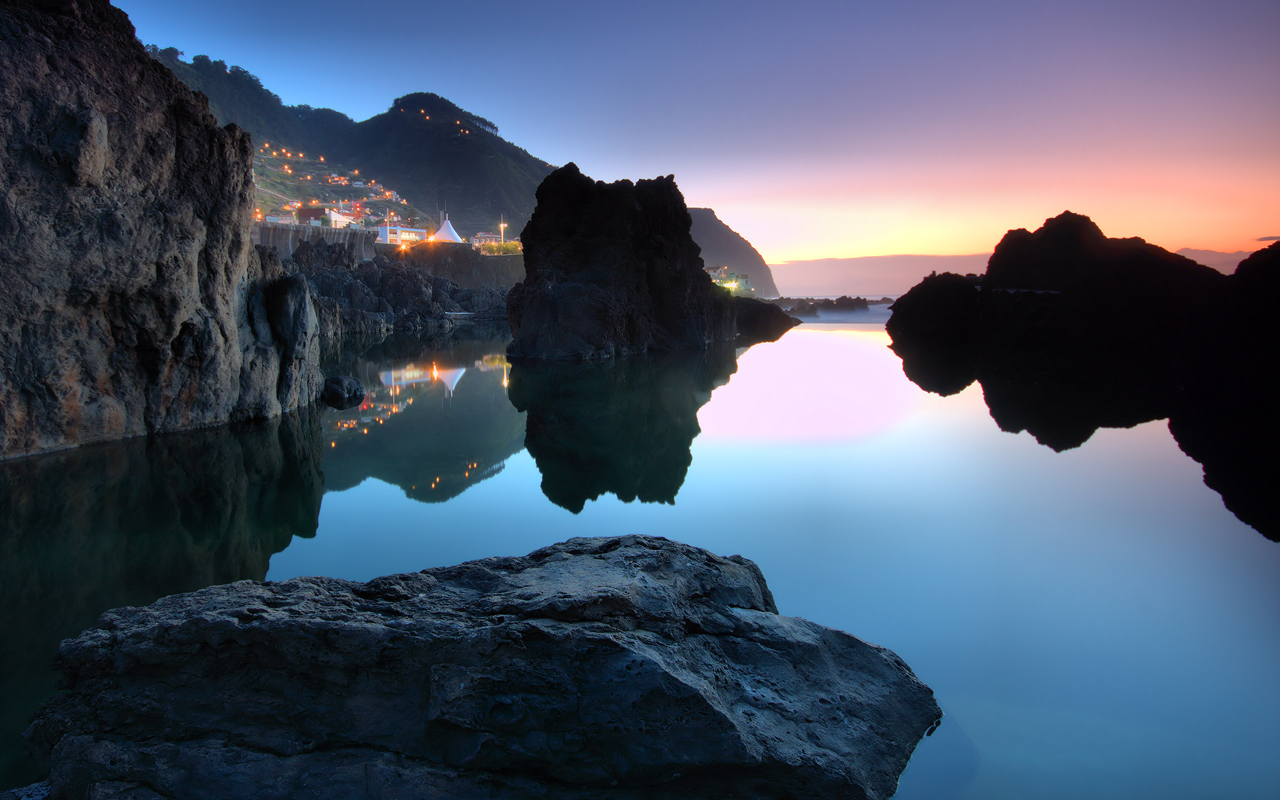
\includegraphics[width=1\linewidth,bb=0 0 1280 800]{portomoniz.jpg}
\caption{The town of Porto Moniz}
\end{figure}

\subsection{Speedup vs. Grain Size}

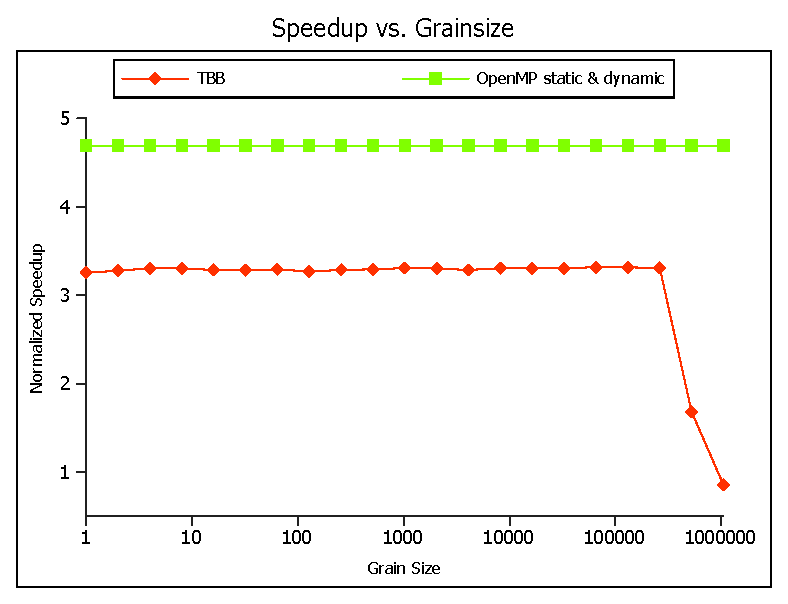
\includegraphics[width=1\linewidth]{graph_grainsize}

As expected, TBB produce a somewhat ideal speedup until grain size got too large for to be evenly
distributed evenly over the number of cores. Surprisingly, OpenMP exhibits super-linear speedup
with the static and dynamic scheduler. Either the grainsize configuration didn't work, or
static values were prechosen, since varying grain size did not significantly affect grainsize.

\subsection{Speedup vs. Number of Particles}
\subsection{Speedup vs. Number of Cores}
\subsection{Speedup vs. Number of Clusters}

\section{Discussion of Results}

\section{Conclusion}

% needed in second column of first page if using \pubid
%\pubidadjcol

% trigger a \newpage just before the given reference
% number - used to balance the columns on the last page
% adjust value as needed - may need to be readjusted if
% the document is modified later
%\IEEEtriggeratref{8}
% The "triggered" command can be changed if desired:
%\IEEEtriggercmd{\enlargethispage{-5in}}
% references section
%\bibliographystyle{IEEEtran.bst}
%\bibliography{IEEEabrv,../bib/paper}
\begin{thebibliography}{1}

\bibitem{IEEEhowto:kopka}
H.~Kopka and P.~W. Daly, \emph{A Guide to {\LaTeX}}, 3rd~ed.
Harlow, England: Addison-Wesley, 1999.

\end{thebibliography}

% biography section
% 
%\begin{biographynophoto}{Chris Jordan}
%Biography text here.
%\end{biographynophoto}

% if you will not have a photo
%\begin{biographynophoto}{Victor Janmey}
%Biography text here.
%\end{biographynophoto}

% insert where needed to balance the two columns on the last page
%\newpage

%\begin{biographynophoto}{Raymond Ko}
%Biography text here.
%\end{biographynophoto}

% You can push biographies down or up by placing
% a \vfill before or after them. The appropriate
% use of \vfill depends on what kind of text is
% on the last page and whether or not the columns
% are being equalized.

%\vfill

% Can be used to pull up biographies so that the bottom of the last one
% is flush with the other column.
%\enlargethispage{-5in}

\end{document}
